% -*- TeX -*-
%
% ----------------------------------------------------------------------
%
%                           Brad T. Aagaard
%                        U.S. Geological Survey
%
% {LicenseText}
%
% ----------------------------------------------------------------------
%

\documentclass{beamer}
\usepackage{amsmath}
\usepackage{array}
\usepackage{mpmulti}

\title{CIG PyLith Tutorial Workshop}
\subtitle{}
\author{Brad Aagaard \\
  Charles Williams \\
  Matt Knepley}
\institute{}
\date{May 17, 2011}


% ---------------------------------------------------- CUSTOMIZATION
\newcommand{\thispdfpagelabel}[1]{}
\newcommand{\newfeature}[1]{{\color{blue}#1}}
\usetheme{CIG}

% ========================================================= DOCUMENT
\begin{document}

% ------------------------------------------------------------ SLIDE
\maketitle

% ------------------------------------------------------------ SLIDE
\logo{\includegraphics[height=4.5ex]{../../logos/cig}}

% ========================================================== SECTION
\section{Introduction}
\subsection{Agenda}

% ------------------------------------------------------------ SLIDE
\begin{frame}
  \frametitle{Workshop Agenda}
  \summary{}

  \begin{center}
    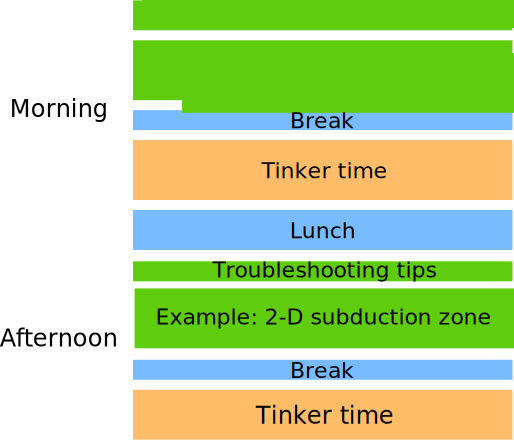
\includegraphics[height=2.9in]{figs/overview}
  \end{center}
  
\end{frame}

% ========================================================== SECTION
\subsection{CIG}

% ------------------------------------------------------------ SLIDE
\begin{frame}
  \frametitle{What is CIG?}
  \summary{Computational Infrastructure for Geodynamics
    ({\tt www.geodynamics.org})}
 
  \vfill

  Objective: Develop, support, and disseminate software for the
  geodynamics community.

  \vfill

  \begin{itemize}
  \item Coordinated effort to develop reusable, well-documented,
    open-source geodynamics software
  \item Strategic partnerships with the larger world of
    computational science and geoinformatics
  \item Specialized training and workshops for both geodynamics and
    larger Earth-science communities
  \end{itemize}

  \vfill
 
  Underlying principle: Earth scientists need help from computational
  scientists to develop state-of-the-art modeling codes

\end{frame}


% ------------------------------------------------------------ SLIDE
\begin{frame}
  \frametitle{CIG: Institution-Based Organization}
  \summary{Educational and not-for-profit organization}
 
  \begin{itemize}
  \item {\bf Open-organization}
    \begin{itemize}
    \item Any institution seeking to collaborate on the development of
      open-source geodynamics software
    \item No cost or size requirements
    \end{itemize}
  \item Current members
    \begin{itemize}
    \item 50 member institutions
    \item 10 foreign affiliates
    \end{itemize}
  \item NSF funding Jul 2010 -- Jun 2015
 \end{itemize}
\end{frame}


% ------------------------------------------------------------ SLIDE
\begin{frame}
  \frametitle{CIG Working Groups}
  \summary{Organized by sub-disciplines}
 
 \begin{itemize}
 \item Short-term tectonics
 \item Long-term tectonics
 \item Mantle convection
 \item Computational seismology
 \item Geodynamo
 \item Magma dynamics
 \end{itemize}

\end{frame}


% ------------------------------------------------------------ SLIDE
\begin{frame}
  \frametitle{Short-Term Tectonics Working Group}
  \summary{}
 
 \vfill
 
 \textbf{Objective}: Simulate crustal deformation across spatial
 scales from $1$ m to $10^3$ km and temporal scales ranging from
 $0.01$ s to $10^5$ years.

 \vfill
 \begin{itemize}
 \item Formed through efforts by Brad Hager and Mark Simons before CIG started
 \item Strong connection to SCEC Crustal Deformation Modeling focus group
 \item Building connections with SCEC Earthquake Source Physics focus group
 \end{itemize}
\vfill

\end{frame} 


% ------------------------------------------------------------ SLIDE
\begin{frame}
  \frametitle{CIG Organizational Structure}
  \summary{}
 
  \begin{itemize}
  \item Staff
    \begin{itemize}
    \item Responsible for software development
    \item Director handles day-to-day decisions
    \end{itemize}
  \item Science Steering Committee
    \begin{itemize}
    \item Voice of geophysics community
    \item Prioritizes the competing needs of all sub-disciplines
    \end{itemize}
  \item Executive Committee
    \begin{itemize}
    \item Primary decision-making body
    \item Approves SSC recommendations and contractual arrangements
    \end{itemize}
  \item Member institution representatives
    \begin{itemize}
    \item Vote on membership applications and bylaws
    \end{itemize}
  \item Community members
    \begin{itemize}
    \item Collaborate with staff to develop software
    \end{itemize}
  \end{itemize}

\end{frame}

% ------------------------------------------------------------ SLIDE
\begin{frame}
  \frametitle{CIG Activities}
  \summary{}

  \begin{itemize}
  \item Software development: primary activity
  \item Workshops
    \begin{itemize}
    \item Sponsors workshops organized by one or more working groups
    \item Holds workshops focusing on scientific computing and geodynamics
    \end{itemize}
  \item Training in use of CIG software
    \begin{itemize}
    \item Tutorials at workshops
    \item Specialized training sessions (like this one)
    \end{itemize}
  \item Web site: {\tt geodynamics.org}
    \begin{itemize}
    \item Distribution of software and documentation
    \item Mailing lists for each working group
    \item Wiki-like web pages for community involvement
    \end{itemize}
  \end{itemize}
 
\end{frame}


% ------------------------------------------------------------ SLIDE
\begin{frame}
  \frametitle{CIG Software}
  \summary{}

  \vfill
  \begin{center}
    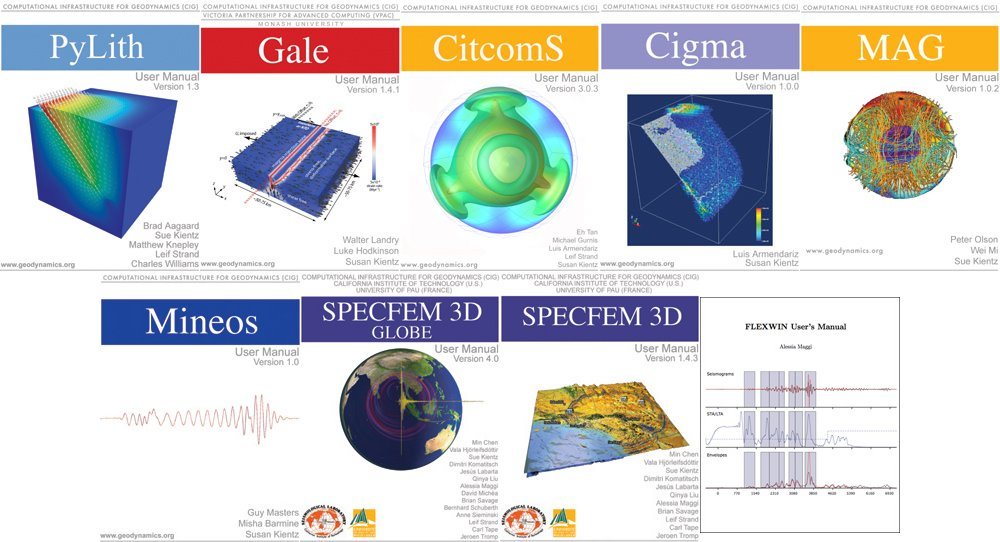
\includegraphics[width=4.5in]{figs/covers}
  \end{center}
  \vfill

\end{frame}

% ------------------------------------------------------------ SLIDE
\begin{frame}
  \frametitle{CIG Software for Crustal Deformation}
  \summary{}

  \begin{itemize}
  \item PyLith
    \begin{itemize}
    \item Solves 2-D and 3-D problems associated with earthquake
      faulting and quasi-static and dynamic viscoelastic deformation
    \item Short-term tectonics where geometry does not change
      significantly
    \end{itemize}
  \item Gale
    \begin{itemize}
    \item Solves problems in orogenesis, rifting, and subduction,
      including free surfaces with coupling to surface erosion models
    \item Long-term tectonics where geometry changes significantly
    \end{itemize}
  \end{itemize}
 
\end{frame}


% ========================================================== SECTION
\section{PyLith}
\subsection{Overview}

% ------------------------------------------------------------ SLIDE
\begin{frame}
  \frametitle{Crustal Deformation Modeling}
  \summary{Elasticity problems where geometry does not change significantly}

  \vfill
  Quasistatic modeling associated with earthquakes
  \vfill

  \begin{itemize}
  \item Strain accumulation associated with interseismic deformation
    \begin{itemize}
    \item What is the stressing rate on faults X, Y, and Z?
    \item Where is strain accumulating in the crust?
    \end{itemize}
  \item Coseismic stress changes and fault slip
    \begin{itemize}
    \item What was the slip distribution in earthquake A?
    \item How did earthquake A change the stresses on faults X, Y, and Z?
    \end{itemize}
  \item Postseismic relaxation of the crust
    \begin{itemize}
    \item What rheology is consistent with observed postseismic deformation?
    \item Can aseismic creep or afterslip explain the deformation?
    \end{itemize}
  \end{itemize}
  \vfill

\end{frame}


% ------------------------------------------------------------ SLIDE
\begin{frame}
  \frametitle{Crustal Deformation Modeling}
  \summary{Elasticity problems where geometry does not change significantly}

  \vfill
  Dynamic modeling associated with earthquakes
  \vfill

  \begin{itemize}
  \item Modeling of strong ground motions
    \begin{itemize}
    \item Forecasting the amplitude and spatial variation in ground
      motion for scenario earthquakes
    \end{itemize}
  \item Coseismic stress changes and fault slip
    \begin{itemize}
    \item How did earthquake A change the stresses on faults X, Y, and Z?
    \end{itemize}
  \item Earthquake rupture behavior
    \begin{itemize}
    \item What fault constitutive models/parameters are consistent
      with the observed rupture propagation in earthquake A?
    \end{itemize}
  \end{itemize}
  \vfill

\end{frame}


% ------------------------------------------------------------ SLIDE
\begin{frame}
  \frametitle{Crustal Deformation Modeling}
  \summary{Elasticity problems where geometry does not change significantly}

  \vfill
  Volcanic deformation associated with magma chambers and/or dikes
  \begin{itemize}
  \item Inflation
    \begin{itemize}
    \item What is the geometry of the magma chamber?
    \item What is the potential for an eruption?
    \end{itemize}
  \item Eruption
    \begin{itemize}
    \item Where is the deformation occurring?
    \item What is the ongoing potential for an eruption?
    \end{itemize}
  \item Dike intrusions
    \begin{itemize}
    \item What the geometry of the intrusion?
    \end{itemize}
  \end{itemize}
  \vfill

\end{frame}


% ------------------------------------------------------------ SLIDE
\begin{frame}
  \frametitle{PyLith}
  \summary{}

  \begin{itemize}
  \item Developers
    \begin{itemize}
    \item Brad Aagaard (USGS, lead developer))
    \item Charles Williams (GNS Science, formerly at RPI)
    \item Matthew Knepley (Univ. of Chicago, formerly at ANL)
    \end{itemize}
  \item Combined dynamic modeling capabilities of EqSim (Aagaard) with
    the quasistatic modeling capabilities of Tecton (Williams)
  \item Use modern software engineering (modular design, testing,
    documentation, distribution) to develop an open-source, community code
  \end{itemize}

\end{frame}


% ------------------------------------------------------------ SLIDE
\begin{frame}
  \frametitle{Crustal Deformation Modeling}
  \summary{Overview of workflow for typical research problem}

  \vfill
  \begin{center}
    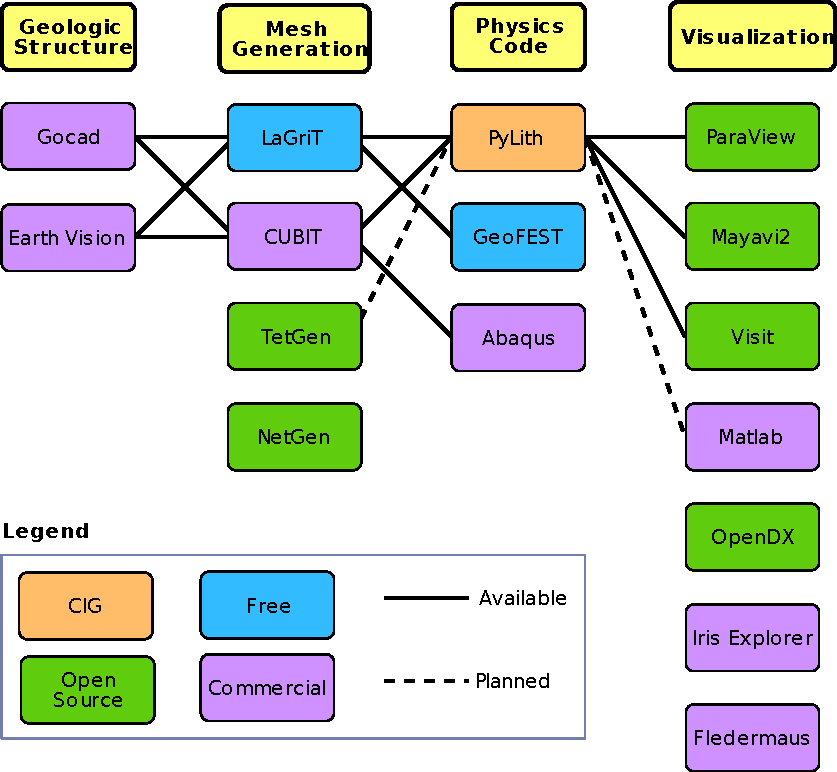
\includegraphics[height=2.9in]{figs/workflow}
  \end{center}
  \vfill

\end{frame}


% ========================================================== SECTION
\subsection{Governing Equations}

% ------------------------------------------------------------ SLIDE
\begin{frame}
  \frametitle{Governing Equations}
  \summary{}

  \vfill
  Elasticity equation
  \begin{gather}
    \sigma_{ij,j} + f_i = \rho \ddot{u} \text{ in } V, \\
    \sigma_{ij} n_j = T_i \text{ on } S_T, \\
    u_i = u_i^0 \text{ on } S_u, \text{ and } \\
    R_{ki}(u^{+}_i - u^{-}_i) = d_k \text{ on } S_f.
  \end{gather}
  Multiply by weighting function and integrate over the volume,
  \begin{equation}
    -\int_V (\sigma_{ij,j} + f_i - \rho \ddot{u}_i) \phi_i \, dV = 0
  \end{equation}
  After some algebra,
  \begin{equation}
    -\int_V \sigma_{ij} \phi_{i,j} \, dV 
    + \int_{S_T} T_i \phi_i\, dS
    + \int_V f_i \phi_i \, dV 
    - \int_V \rho \ddot{u}_i \phi_i \, dV = 0
  \end{equation}
  \vfill
  
\end{frame}


% ------------------------------------------------------------ SLIDE
\begin{frame}
  \frametitle{Governing Equations}
  \summary{}

  \vfill
  Writing the trial and weighting functions in terms of basis (shape)
  functions,
  \begin{gather}
    u_i(x_i, t) = \sum_m a^m_i(t) N^m(x_i), \\
    \phi_i(x_i, t) = \sum_n c^n_i(t) N^n(x_i).
  \end{gather}
  After some algebra, the equation for degree of freedom $i$ of
  vertex $n$ is
  \begin{multline}
    -\int_V \sigma_{ij} N^n_{,j} \, dV 
    + \int_{S_T} T_i N^n \, dS
    + \int_V f_i N^n \, dV 
    - \int_V \rho \sum_m \ddot{a}^m_i N^m N^n \, dV = 0
  \end{multline}
  \vfill

\end{frame}

% ------------------------------------------------------------ SLIDE
\begin{frame}
  \frametitle{Governing Equations}
  \summary{}

  Using numerical quadrature we convert the integrals to sums over the
  cells and quadrature points
  \begin{multline}
    -\sum_\text{vol cells} \sum_\text{quad pts} \sigma_{ij} N^n_{,j} w_q |J_\text{cell}|
    + \sum_\text{surf cells} \sum_\text{quad pts} T_i N^n w_q |J_\text{cell}|\\
    + \sum_\text{vol cells} \sum_\text{quad pts}  f_i N^n w_q |J_\text{cell}|\\
    - \sum_\text{vol cells} \sum_\text{quad pts} \rho \sum_m \ddot{a}^m_i N^m N^n w_q |J_\text{cell}| = \vec{0}    
  \end{multline}

\end{frame}


% ------------------------------------------------------------ SLIDE
\begin{frame}
  \frametitle{Quasistatic Solution}
  \summary{Neglect inertial terms}

  \vfill
  Form system of algebraic equations
  \begin{equation}
    \underline{A} (t) \vec{u}(t) = \vec{b}(t)
  \end{equation}
  where
  \begin{gather}
    A^{nm}_{ij}(t) = \sum_\text{vol cells} \sum_\text{quad pts} 
      \frac{1}{4} C_{ijkl}(t) (N^m_{,l} + N^m_{,k})(N^n_{,j} + N^n_{,i}) w_q |J_\text{cell}| \\
    b_i(t) =    
     \sum_\text{surf cells} \sum_\text{quad pts} T_i(t) N^n w_q |J_\text{cell}| 
    + \sum_\text{vol cells} \sum_\text{quad pts}  f_i(t) N^n w_q |J_\text{cell}|
\end{gather}
  and solve for $\vec{u}(t)$.
  \vfill


\end{frame}


% ========================================================== SECTION
\subsection{Fault Implementation}

% ------------------------------------------------------------ SLIDE
\begin{frame}
  \frametitle{Implementation: Fault Interfaces}
   \summary{Use cohesive cells to control fault behavior}
 
   \vfill
   \begin{center}
     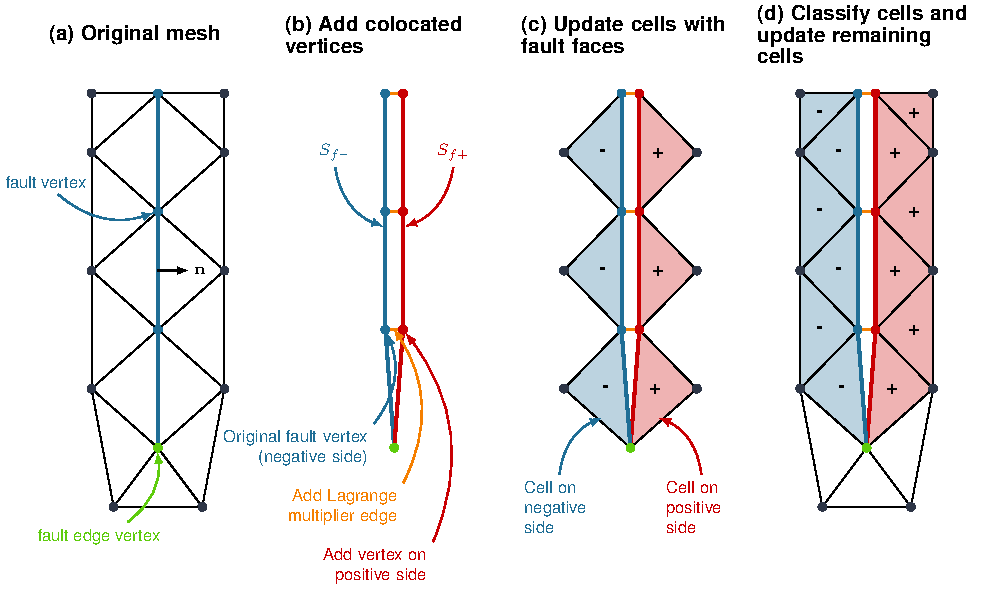
\includegraphics[width=4.5in]{figs/cohesivecells}
   \end{center}
   
 \end{frame}
 

% ------------------------------------------------------------ SLIDE
\begin{frame}
  \frametitle{Fault Slip Implementation}
  \summary{Use Lagrange multipliers to specify slip}

  \begin{itemize}
  \item System without cohesive cells
    \begin{itemize}
    \item Conventional finite-element elasticity formulation
      \begin{equation}
        \underbar{A} \vec{u} = \vec{b} \nonumber
      \end{equation}
    \item Fault slip associated with relative displacements across fault
      \begin{equation}
        \underbar{C} \vec{u} = \vec{d} \nonumber
      \end{equation}
    \end{itemize}
  \item System with cohesive cells
    \begin{equation}
      \left( \begin{array}{cc}
          \underbar{A} & \underbar{C}^T\\
          \underbar{C} & 0
        \end{array} \right)
      \left( \begin{array}{c}
          \vec{u}\\
          \vec{l}
        \end{array}\right)
      =
      \left( \begin{array}{c}
          \vec{b}\\
          \vec{d}
        \end{array} \right)
      \nonumber
    \end{equation}
  \item Lagrange multipliers are tractions associated with fault slip
  \item Prescribed (kinematic) slip\\
    Specify fault slip ($\vec{d}$) and solve for Lagrange multipliers ($\vec{l}$)
  \item Spontaneous (dynamic) slip\\
    Adjust fault slip to be compatible with fault constitutive model
\end{itemize}
  
\end{frame}


% ------------------------------------------------------------ SLIDE
\begin{frame}
  \frametitle{Implementing Fault Slip with Lagrange multipliers}
 
 \begin{itemize}
 \item Advantages
   \begin{itemize}
   \item Fault implementation is local to cohesive cell
   \item Solution includes forces generating slip (Lagrange multipliers)
   \item Retains block structure of matrix, including symmetry
   \item Offsets in mesh mimic slip on natural faults
   \end{itemize}
 \item Disadvantages 
   \begin{itemize}
   \item Cohesive cells require adjusting topology of finite-element mesh
  \end{itemize}
 \end{itemize}
  
\end{frame}


% ========================================================== SECTION
\subsection{Running PyLith}

% ------------------------------------------------------------ SLIDE
\begin{frame}
  \frametitle{Ingredients for Running PyLith}

  \begin{itemize}
  \item Simulation parameters
  \item Finite-element mesh
    \begin{itemize}
    \item Mesh exported from LaGriT
    \item Mesh exported from CUBIT
    \item Mesh constructed by hand (PyLith mesh ASCII format)
    \end{itemize}
  \item Spatial databases for physical properties, boundary
    conditions, and rupture parameters
    \begin{itemize}
    \item SCEC CVM-H or USGS Bay Area Velocity model
    \item Simple ASCII files
    \end{itemize}
  \end{itemize}

\end{frame}


% ------------------------------------------------------------ SLIDE
\begin{frame}
  \frametitle{Spatial Databases}
  \summary{User-specified field/value in space}

  \begin{itemize}
 \item Examples
    \begin{itemize}
    \item Uniform value for Dirichlet (0-D)
    \item Piecewise linear variation in tractions for Neumann BC (1-D)
    \item SCEC CVM-H seismic velocity model (3-D)
    \end{itemize}
  \item Generally independent of discretization for problem
  \item Available spatial databases
    \begin{description}
    \item[UniformDB] Optimized for uniform value
    \item[SimpleDB] Simple ASCII files (0-D, 1-D, 2-D, or 3-D)
    \item[SCECCVMH] SCEC CVM-H seismic velocity model v5.3
    \item[ZeroDispDB] Special case of UniformDB
    \end{description}
 \end{itemize}

\end{frame}


% ========================================================== SECTION
\subsection{Features}

% ------------------------------------------------------------ SLIDE
\begin{frame}
  \frametitle{Features in PyLith 1.5}
  \summary{Enhancements and new features in \newfeature{blue}}

  \begin{itemize}
  \item Time integration schemes and elasticity formulations
    \begin{itemize}
    \item Implicit for quasistatic problems (neglect inertial terms)
      \begin{itemize}
      \item Infinitesimal strains
      \item \newfeature{Small strains}
      \end{itemize}
    \item Explicit for dynamic problems
      \begin{itemize}
      \item Infinitesimal strains with sparse system Jacobian
      \item \newfeature{Infinitesimal strains with lumped system Jacobian}
      \item \newfeature{Small strains with sparse system Jacobian}
      \end{itemize}
    \end{itemize}
  \item Bulk constitutive models
    \begin{itemize}
    \item Elastic model (1-D, 2-D, and 3-D)
    \item Linear and Generalized Maxwell viscoelastic models (3-D)
    \item Power-law viscoelastic model (3-D)
    \item \newfeature{Linear Maxwell viscoelastic model (2-D)}
    \item \newfeature{Drucker-Prager elastoplastic model (3-D)}
    \end{itemize}
 \end{itemize}

\end{frame}


% ------------------------------------------------------------ SLIDE
\begin{frame}
  \frametitle{Features in PyLith 1.5 (cont.)}
  \summary{Enhancements and new features in \newfeature{blue}}

  \begin{itemize}
  \item Boundary and interface conditions
    \begin{itemize}
    \item Time-dependent Dirichlet boundary conditions
    \item Time-dependent Neumann (traction) boundary conditions
    \item Absorbing boundary conditions
    \item Kinematic (prescribed slip) fault interfaces w/multiple ruptures
    \item \newfeature{Dynamic (friction) fault interfaces}
    \item Time-dependent point forces
    \item Gravitational body forces
    \end{itemize}
  \item Fault constitutive models
    \begin{itemize}
    \item \newfeature{Static friction}
    \item \newfeature{Linear slip-weakening}
    \item \newfeature{Dieterich-Ruina rate and state friction w/ageing
      law}
   \end{itemize}
 \end{itemize}

\end{frame}


% ------------------------------------------------------------ SLIDE
\begin{frame}
  \frametitle{Features in PyLith 1.5 (cont.)}
  \summary{Enhancements and new features in \newfeature{blue}}

  \begin{itemize}
  \item Automatic and user-controlled time stepping
  \item Ability to specify initial stress state
  \item Importing meshes
    \begin{itemize}
    \item LaGriT: GMV/Pset
    \item CUBIT: Exodus II
    \item ASCII: PyLith mesh ASCII format (intended for toy problems only)
    \end{itemize}
  \item Output: VTK files
    \begin{itemize}
    \item Solution over volume
    \item Solution over surface boundary
    \item State variables (e.g., stress and strain) for each material
    \item Fault information (e.g., slip and tractions)
    \end{itemize}
  \item Automatic conversion of units for all parameters
  \end{itemize}
  
\end{frame}


% ------------------------------------------------------------ SLIDE
\begin{frame}
  \frametitle{PyLith Development}
  \summary{}

  \begin{itemize}
  \item Long-term priorities
    \begin{itemize}
    \item Multi-cycle earthquake modeling
      \begin{itemize}
      \item Resolve interseismic, coseismic, and postseismic deformation
      \item Elastic/viscoelastic/plastic rheologies
      \item Coseismic slip, afterslip, and creep
      \end{itemize}
   \item Efficient computation of 3-D and 4-D Green's functions
    \item Scaling to 1000 processors
   \end{itemize}
  \item Short-term priorities
    \begin{itemize}
    \item Implement several new feature and improve parallel
      performance
    \item Increase user training using virtual workshops
    \begin{itemize}
      \item CIG/SCEC/NASA/NSF workshop: annual $\rightarrow$ biannual\\
        (Jun 2012)
      \item Jun 20-24, 2011: PyLith traininng via virtual workshop
      \end{itemize}
    \end{itemize}
  \end{itemize}

\end{frame}


% ------------------------------------------------------------ SLIDE
\begin{frame}
  \frametitle{PyLith Development}
  \summary{Planned Releases}

  \begin{itemize}
  \item v1.6 (June 2011)
    \begin{itemize}
    \item HDF5 output (parallel, binary I/O)
    \item Custom preconditioner with AMG solver
    \item Uniform, global mesh refinement
    \item Numerical damping via viscosity for dynamic problems
    \end{itemize}
  \item v1.7 (Fall 2011)
    \begin{itemize}
    \item Accelerate FE integrations using GPUs
    \item Scalable mesh distribution among processors
    \item Attenuation for dynamic simulations (wave propagation)
    \end{itemize}
  \item v2.0 (June 2012)
    \begin{itemize}
    \item Coupling of quasistatic and dynamic simulations
    \item Heat and fluid flow coupled to elastic deformation
    \item Higher order FE basis functions
    \item Moment tensor point sources
    \item Support for incompressible elasticity
   \end{itemize}
  \end{itemize}

\end{frame}


% ========================================================== SECTION
\subsection{Architecture}

% ------------------------------------------------------------ SLIDE
\begin{frame}
  \frametitle{Design Philosophy}
  \summary{Modular, extensible, and smart}

  \begin{itemize}
  \item Code should be flexible and modular
  \item Users should be able to add new features without modifying
    code, for example:
    \begin{itemize}
    \item Boundary conditions
    \item Bulk constitutive models
    \item Fault constitutive models
    \end{itemize}
  \item Input/output should be user-friendly
  \item Top-level code written in Python (expressive, dynamic typing)
  \item Low-level code written in C++ (modular, fast)
\end{itemize}

\end{frame}


% ------------------------------------------------------------ SLIDE
\begin{frame}
  \frametitle{PyLith Design: Focus on Geodynamics}
  \summary{Leverage packages developed by computational scientists}

  \vfill
  \begin{center}
    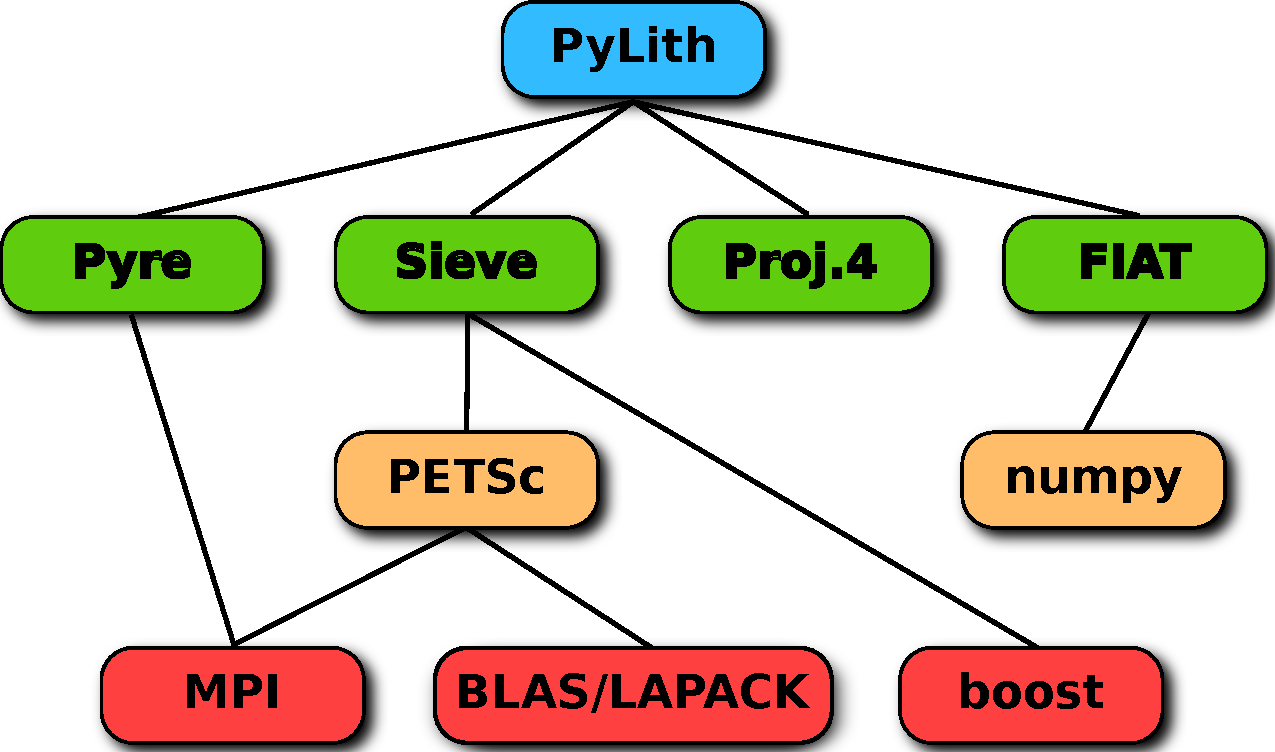
\includegraphics[height=2.5in]{figs/packages}
  \end{center}  
  \vfill

\end{frame}


% ------------------------------------------------------------ SLIDE
\begin{frame}
  \frametitle{PyLith as a Hierarchy of Components}
  \summary{Components are the basic building blocks}

  \vfill
  \begin{center}
    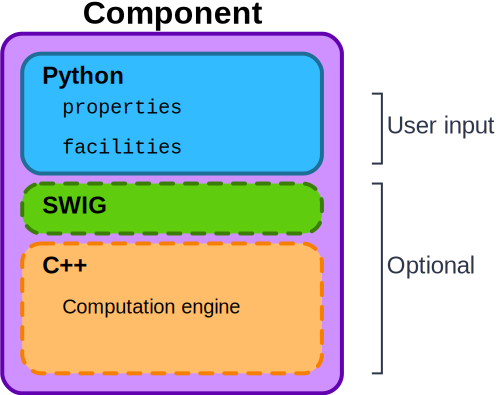
\includegraphics[height=2.0in]{figs/component}
  \end{center}  
  \vfill

\end{frame}


% ------------------------------------------------------------ SLIDE
\begin{frame}
  \frametitle{PyLith as a Hierarchy of Components}
  \summary{PyLith Application and Time-Dependent Problem}

  \vfill
  \begin{center}
    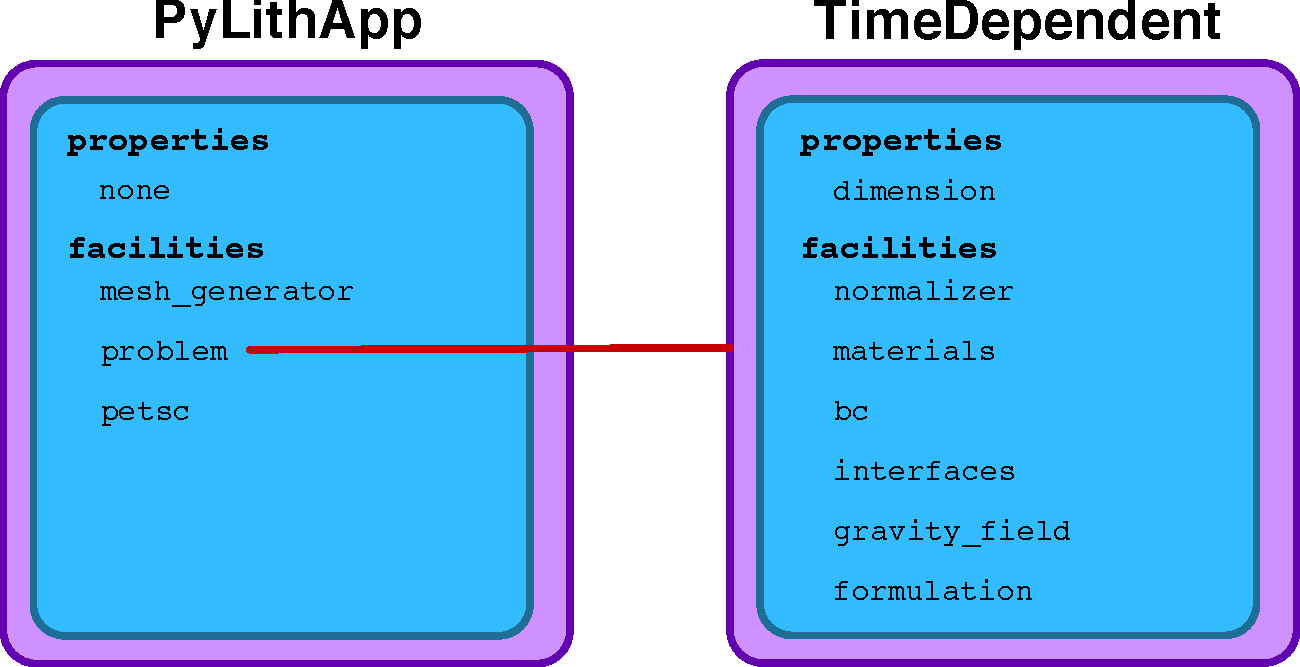
\includegraphics[height=2.0in]{figs/pylithapp}
  \end{center}  
  \vfill

\end{frame}


% ------------------------------------------------------------ SLIDE
\begin{frame}
  \frametitle{PyLith as a Hierarchy of Components}
  \summary{Fault with kinematic (prescribed slip) earthquake rupture}

  \vfill
  \begin{center}
    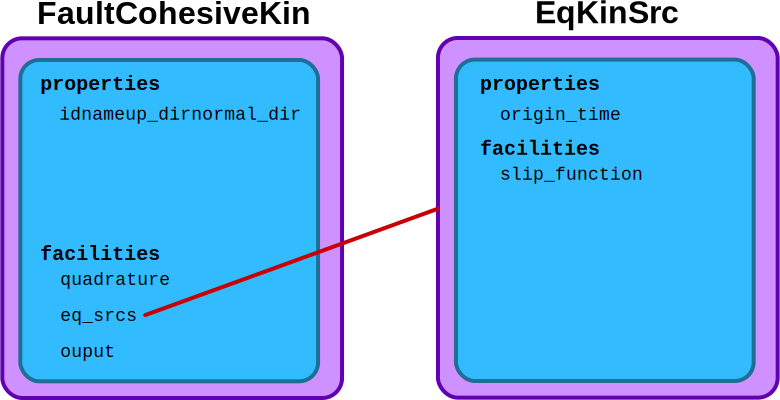
\includegraphics[height=2.0in]{figs/faultcohesivekin}
  \end{center}  
  \vfill

\end{frame}


% ------------------------------------------------------------ SLIDE
\begin{frame}
  \frametitle{PyLith as a Hierarchy of Components}
  \summary{Diagram of simple toy problem}

  \vfill
  \begin{center}
    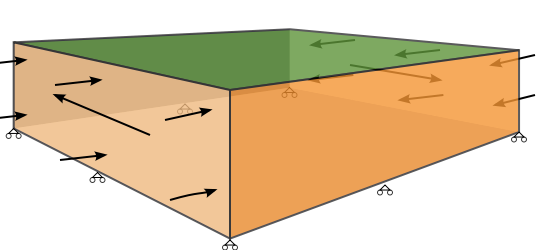
\includegraphics[height=2.0in]{figs/step01_diagram}
  \end{center}  
  \vfill

\end{frame}


% ------------------------------------------------------------ SLIDE
\begin{frame}
  \frametitle{PyLith as a Hierarchy of Components}
  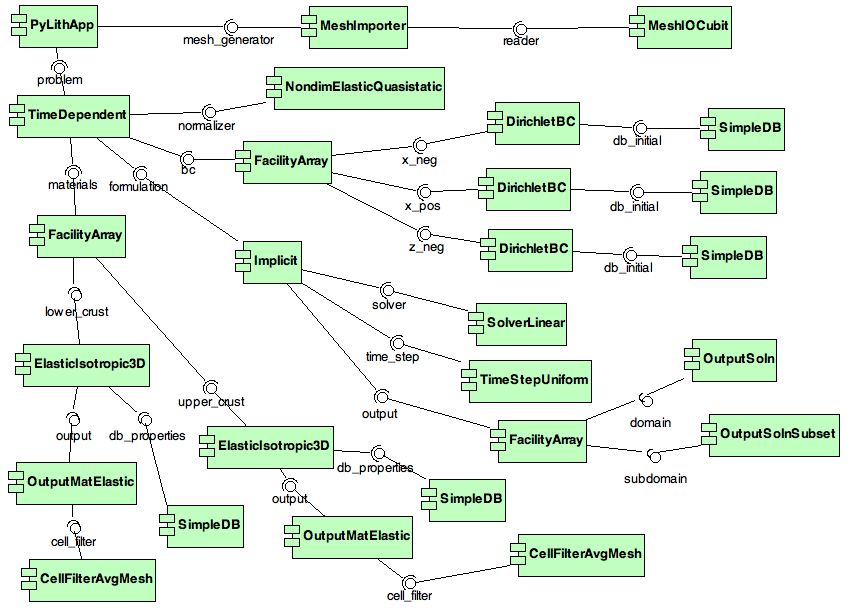
\includegraphics[height=3.2in]{figs/step01_components}
\end{frame}



% ------------------------------------------------------------ SLIDE
\begin{frame}[fragile]
  \frametitle{PyLith Application Flow}
  \summary{}
 
{\small\tt
  \begin{minipage}[t]{2.0in}
      \begin{block}{PyLithApp}
        \begin{verbatim}
main()
  mesher.create()
  problem.initialize()
  problem.run()
\end{verbatim}
    \end{block}
    \begin{block}{TimeDependent (Problem)}
    \begin{verbatim}
initialize()
  formulation.initialize()

run()
  while (t < tEnd)
    dt = formulation.dt()
    formulation.prestep(dt)
    formulation.step(dt)
    formulation.poststep(dt)
\end{verbatim}
  \end{block}
\end{minipage}
  \hfill
  \begin{minipage}[t]{2.0in}
    \begin{block}{Implicit (Formulation)}
      \begin{verbatim}
initialize()

prestep()
  set values of constraints

step()
  compute residual
  solve for disp. incr.

poststep()
   update disp. field
   write output
\end{verbatim}
    \end{block}
  \end{minipage}
}

\end{frame}


% ========================================================== SECTION
\subsection{Testing}

% ------------------------------------------------------------ SLIDE
\begin{frame}
  \frametitle{Unit and Regression Testing}
  \summary{Automatically run more than 1800 tests on multiple
    platforms whenever code is checked into the source repository.}

  \begin{itemize}
  \item Create tests for nearly every function in code during development
    \begin{itemize}
    \item Remove most bugs during initial implementation
    \item Isolate and expose bugs at origin
    \end{itemize}
  \item Create new tests to expose reported bugs
    \begin{itemize}
    \item Prevent bugs from reoccurring
    \end{itemize}
  \item Rerun tests whenever code is changed
    \begin{itemize}
    \item Code continually improves (permits optimization with
      quality control)
    \end{itemize}
  \item Binary packages generated automatically upon successful
    completion of tests
  \item Additional full-scale tests are run before releases
  \end{itemize}

\end{frame}

% ------------------------------------------------------------ SLIDE
\begin{frame}
  \frametitle{Example of Automated Building and Testing}
  \summary{Test written to expose bug, buildbot shows tests fail}

  \begin{center}
    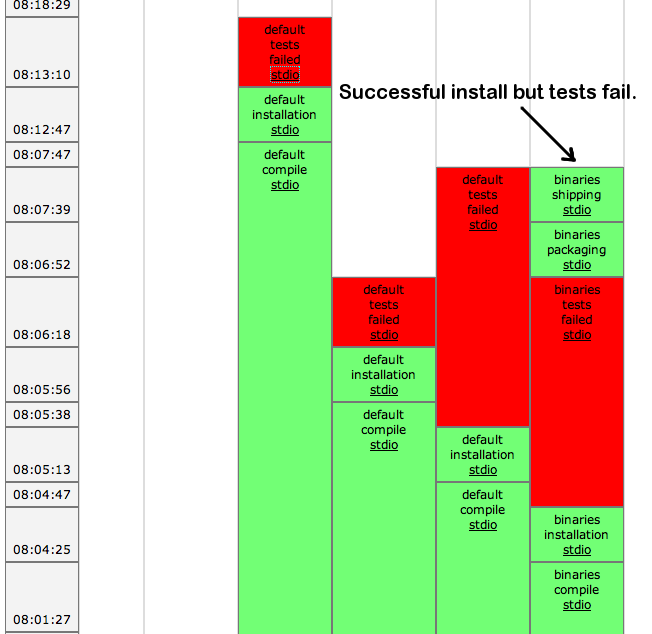
\includegraphics[height=2.9in]{figs/buildbotfail}
  \end{center}

\end{frame}


% ------------------------------------------------------------ SLIDE
\begin{frame}
  \frametitle{Example of Automated Building and Testing}
  \summary{Bug is fixed, buildbot shows tests pass}

  \begin{center}
    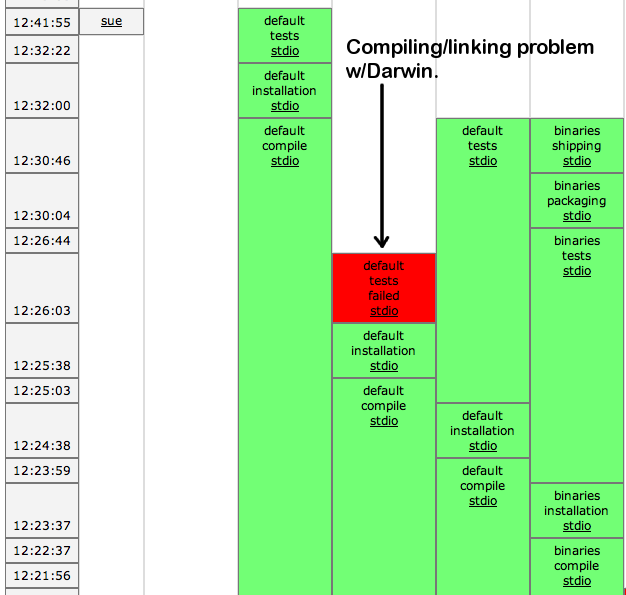
\includegraphics[height=2.9in]{figs/buildbotsuccess}
  \end{center}

\end{frame}

% ======================================================================
\end{document}


% End of file
